\chapter{सांख्यिकीय ऊष्मागतिकी: विभाजन फलन}\label{ch:b3:partition-functions}

वियना में लुडविग बोल्ट्समान की समाधि पर एक ही पंक्ति अंकित है, $S = k\log W$: किसी
निकाय की एन्ट्रॉपी उन तरीकों को गिनती है जिनसे उसके अणु उसकी ऊर्जा आपस में बाँट सकते हैं।
ऊष्मागतिकी, जैसी प्रथम और द्वितीय वर्ष के खंडों ने उसे बनाया, को कभी
अणुओं की आवश्यकता नहीं होती: वह मापी गई ऊष्माओं, एन्ट्रॉपियों और साम्य स्थिरांकों को
परस्पर जोड़ती है। सांख्यिकीय ऊष्मागतिकी उन्हें स्वयं अणुओं से परिकलित करती है।
उसकी केंद्रीय वस्तु एक अणु के ऊर्जा स्तरों पर एक ही योग है, विभाजन फलन;
स्तर स्पेक्ट्रमिकी से आते हैं, और नाइट्रोजन के स्पेक्ट्रम से परिकलित मानक एन्ट्रॉपी
सारणीबद्ध मान से प्रति केल्विन प्रति मोल एक जूल के सौवें भाग तक मेल खाती है। यह अध्याय
विभाजन फलन बनाता है, उसे उसके स्थानांतरणीय, घूर्णी,
कंपनिक और इलेक्ट्रॉनिक भागों में विभक्त करता है, और उसे आंतरिक ऊर्जा, एन्ट्रॉपी
और गिब्स ऊर्जा में बदलता है; \cref{ch:b3:statistical-thermo-applied} उसे ऊष्मा
धारिताओं और साम्य स्थिरांकों पर लागू करता है।

\begin{recall}
द्वितीय वर्ष के खंड ने मानक मोलर एन्ट्रॉपी, गिब्स ऊर्जा और
रासायनिक विभव परिभाषित किए, और निम्न ताप तक मापी गई ऊष्मा धारिताओं से प्राप्त
एन्ट्रॉपियाँ सारणीबद्ध कीं। \Cref{ch:b3:quantum-model-systems} ने \omterm{def:b3:quantum-model-systems:box}{डिब्बे में कण},
\omterm{def:b3:quantum-model-systems:oscillator}{आवर्ती दोलित्र} और \omterm{def:b3:quantum-model-systems:rotor}{दृढ़ घूर्णक} के ऊर्जा स्तर दिए, $E_J = hcBJ(J+1)$, \omterm{def:b3:quantum-model-systems:degenerate}{अपभ्रष्टता} $2J + 1$ के साथ;
\cref{ch:b3:rovibrational-spectroscopy} ने द्विपरमाणुक
अणुओं के लिए $B$ और $\tilde\nu$ मापे और पाया कि \ce{N2} जैसे समनाभिकीय अणु में
नाभिकीय चक्रण एकांतर घूर्णी स्तरों को असमान बना देते हैं।
\end{recall}

\section{सूक्ष्म अवस्थाएँ और बोल्ट्समान वितरण}

$N$ सर्वसम, स्वतंत्र अणुओं पर विचार कीजिए जो ऊर्जा
$\varepsilon_0 = 0 < \varepsilon_1 < \varepsilon_2 < \dots$ वाले स्तरों में रह सकते हैं, कुल ऊर्जा $E$ के साथ। यह बताना कि हर स्तर पर कितने
अणु हैं, $\{n_0, n_1, \dots\}$, एक वितरण का वर्णन करता है;
यह बताना कि कौन-सा अणु किस स्तर पर है, कहीं अधिक का वर्णन करता है।

\begin{definition}[सूक्ष्म अवस्था, सांख्यिकीय भार]\label{def:b3:partition-functions:microstate}
अणुओं के किसी निकाय की \emph{सूक्ष्म अवस्था}\index{सूक्ष्म अवस्था} हर अणु की
अवस्था का पूर्ण विनिर्देश है। \emph{सांख्यिकीय भार}\index{सांख्यिकीय भार} $W$, किसी वितरण
$\{n_i\}$ का, जिसमें $N$ अणु अनपभ्रष्ट स्तरों पर बँटे हैं,
उन सूक्ष्म अवस्थाओं की संख्या है जो उसे साकार करती हैं:
\[
  W = \frac{N!}{n_0!\,n_1!\,n_2!\cdots}.
\]
\end{definition}

\begin{example}[तीन दोलित्रों में तीन क्वांटम]\label{ex:b3:partition-functions:three-quanta}
तीन दोलित्र ऊर्जा के तीन क्वांटम बाँटते हैं। वितरण ``एक
दोलित्र तीनों रखता है'' $3!/(1!\,2!) = 3$ तरीकों से साकार हो सकता है, ``एक
दो रखता है, दूसरा एक'' $3! = 6$ तरीकों से, और ``हर एक एक रखता है'' एक तरीके से:
कुल दस \omterm{def:b3:partition-functions:microstate}{सूक्ष्म अवस्थाएँ}, और सबसे समान वितरण, जो फिर भी ऊर्जा को
कई स्तरों पर फैलाता है, सबसे प्रायिक है। $10^{23}$ अणुओं के साथ
भार इतने तीक्ष्ण शिखर वाले हो जाते हैं कि एक वितरण, और उससे नगण्य मात्रा में
भिन्न वितरण, व्यावहारिक रूप से सभी \omterm{def:b3:partition-functions:microstate}{सूक्ष्म अवस्थाएँ} वहन करते हैं।
\end{example}

\begin{remark}
सांख्यिकीय ऊष्मागतिकी का अभिगृहीत यह है कि दी हुई ऊर्जा वाले किसी विलगित
निकाय की सभी \omterm{def:b3:partition-functions:microstate}{सूक्ष्म अवस्थाएँ} समप्रायिक हैं। तब निकाय, अत्यधिक संभावना से,
सबसे बड़े भार वाले वितरण में पाया जाता है: उसे ज्ञात करना
इस अनुभाग का कार्य है।
\end{remark}

बड़ी संख्याओं के लिए स्टर्लिंग सन्निकटन $\ln x! \approx x\ln x - x$ यह देता है:
\[
  \ln W = N\ln N - \sum_i n_i\ln n_i .
\]

\begin{definition}[बोल्ट्समान वितरण, समष्टि]\label{def:b3:partition-functions:boltzmann}
किसी स्तर की \emph{समष्टि}\index{समष्टि} $n_i/N$ उन अणुओं का अंश है जो
उस स्तर में हैं। \emph{बोल्ट्समान वितरण}\index{बोल्ट्समान वितरण}
ताप $T$ पर तापीय साम्य में स्वतंत्र अणुओं का सबसे बड़े भार वाला वितरण है,
जो नीचे के प्रमेय द्वारा दिया गया है।
\end{definition}

\begin{theorem}[बोल्ट्समान वितरण]\label{thm:b3:partition-functions:boltzmann}
ताप $T$ पर साम्य में स्वतंत्र अणुओं के लिए, ऊर्जा $\varepsilon_i$ और
\omterm{def:b3:quantum-model-systems:degenerate}{अपभ्रष्टता} $g_i$ वाले स्तर की \omterm{def:b3:partition-functions:boltzmann}{समष्टि} यह है:
\[
  \frac{n_i}{N} = \frac{g_i\eu^{-\varepsilon_i/kT}}{q},
  \qquad q = \sum_i g_i\eu^{-\varepsilon_i/kT},
\]
जहाँ $k$ बोल्ट्समान स्थिरांक है। दो स्तरों की \omterm{def:b3:partition-functions:boltzmann}{समष्टियों} का अनुपात
$\frac{n_j}{n_i} = \frac{g_j}{g_i}\eu^{-(\varepsilon_j - \varepsilon_i)/kT}$ है।
\end{theorem}

\begin{proof}[आंशिक उपपत्ति]
पहले अनपभ्रष्ट स्तर लीजिए। $\ln W$ को दो प्रतिबंधों
$\sum_in_i = N$ और $\sum_in_i\varepsilon_i = E$ के अधीन, लाग्रांज गुणकों $\alpha$ और $\beta$ के साथ, अधिकतम कीजिए:
हर $i$ के लिए,
\[
  \frac{\partial}{\partial n_i}\Bigl(\ln W + \alpha\sum_jn_j - \beta\sum_jn_j\varepsilon_j\Bigr)
  = -\ln n_i - 1 + \alpha - \beta\varepsilon_i = 0,
\]
अतः $n_i = \eu^{\alpha - 1}\eu^{-\beta\varepsilon_i}$, और पहला प्रतिबंध $\eu^{\alpha - 1}
= N/\sum_j\eu^{-\beta\varepsilon_j}$ निर्धारित करता है। \omterm{def:b3:quantum-model-systems:degenerate}{अपभ्रष्टता} $g_i$ वाला स्तर समान ऊर्जा की $g_i$ भिन्न अवस्थाएँ हैं,
हर एक ऊपर की तरह समष्टित: उसकी \omterm{def:b3:partition-functions:boltzmann}{समष्टि}
$g_i$ से गुणा हो जाती है। गुणक $\beta$ की पहचान एक ज्ञात स्थिति से होती है:
आदर्श गैस की स्थानांतरणीय गति के लिए (\cref{prop:b3:partition-functions:q-trans},
नीचे) वितरण ऊर्जा $\frac32N/\beta$ देता है, और आदर्श-गैस
ऊर्जा $\frac32NkT$ है; अतः $\beta = 1/kT$। यह कि $\beta$ हर प्रकार की गति के लिए
वही राशि है, और कि यह ऊष्मागतिक ताप है, यहाँ स्वीकार किया गया है:
तापीय संपर्क में दो निकाय एक ही $\beta$ साझा करते हैं, जो ताप का परिभाषक
गुणधर्म है।
\end{proof}

\begin{definition}[आण्विक विभाजन फलन]\label{def:b3:partition-functions:partition-function}
ताप $T$ पर किसी अणु का \emph{आण्विक विभाजन फलन}\index{आण्विक विभाजन फलन}
यह योग है:
\[
  q = \sum_{\text{स्तर}}g_i\eu^{-\varepsilon_i/kT} = \sum_{\text{अवस्थाएँ}}\eu^{-\varepsilon_s/kT},
\]
जहाँ ऊर्जाएँ निम्नतम स्तर से मापी जाती हैं, ताकि $q \ge 1$।
\end{definition}

विभाजन फलन उन अवस्थाओं को गिनता है जो तापीय रूप से सुलभ हैं:
बहुत निम्न ताप पर केवल निम्नतम स्तर योगदान देता है और $q \to g_0$; बहुत
ऊँचे ताप पर हर अवस्था लगभग 1 का योगदान देती है और $q$ असीमित बढ़ता है।
इससे एक व्यावहारिक नियम निकलता है: निम्नतम स्तर से $kT$ से बहुत अधिक ऊपर के स्तर
रिक्त होते हैं, उससे $kT$ के भीतर के स्तर समष्टित होते हैं। \qty{298.15}{K} पर $kT$,
\qty{207.2}{cm^{-1}} के संगत है, या $RT = \qty{2.479}{kJ/mol}$।

\begin{method}[स्पेक्ट्रमी स्थिरांकों से स्तरों की समष्टियाँ]\label{met:b3:partition-functions:populations}
\begin{enumerate}
  \item स्तरों को उनकी ऊर्जाओं (स्थिरांकों से, जैसे
        $hcBJ(J+1)$) और \omterm{def:b3:quantum-model-systems:degenerate}{अपभ्रष्टताओं} ($2J + 1$) सहित सूचीबद्ध कीजिए।
  \item हर ऊर्जा को $kT$ की इकाइयों में व्यक्त कीजिए; \qty{298.15}{K} पर किसी
        तरंग-संख्या को \qty{207.2}{cm^{-1}} से भाग दीजिए।
  \item पद $g_i\eu^{-\varepsilon_i/kT}$ बनाइए, उन्हें जोड़कर $q$ प्राप्त कीजिए, और भाग दीजिए।
        जब पद नगण्य हो जाएँ तो योग रोक दीजिए।
  \item जाँच: \omterm{def:b3:partition-functions:boltzmann}{समष्टियों} का योग 1 है; उनमें से दो का अनुपात
        $\frac{g_j}{g_i}\eu^{-(\varepsilon_j-\varepsilon_i)/kT}$ है।
\end{enumerate}
\end{method}

\begin{example}[हाइड्रोजन क्लोराइड के घूर्णी स्तर]\label{ex:b3:partition-functions:hcl}
% ledger: diat:HCl.Be, diat:HCl.ae
\ce{H^{35}Cl} के लिए $B_0 = B_e - \alpha_e/2 = \qty{10.44}{cm^{-1}}$। \qty{300}{K} पर स्तर $J$
$10.44\,J(J+1)$~\unit{cm^{-1}} पर है, अर्थात् $0.0501\,J(J+1)$ पर, $kT$ की इकाइयों में। पद
$(2J+1)\eu^{-0.0501J(J+1)}$ हैं 1, 2.71, 3.70, 3.84, 3.31, 2.45, \dots; उनका योग
$q = 20.3$ है और $J = 0$ से 4 की \omterm{def:b3:partition-functions:boltzmann}{समष्टियाँ} 0.049, 0.134, 0.182, 0.189 और
0.163 हैं: सबसे अधिक समष्टित स्तर $J = 3$ है, $J = 0$ नहीं, क्योंकि \omterm{def:b3:quantum-model-systems:degenerate}{अपभ्रष्टता}
$2J + 1$ बढ़ती है जबकि बोल्ट्समान गुणक घटता है। यही
\cref{ch:b3:rovibrational-spectroscopy} के घूर्णन--कंपन बैंड का आवरण है।
\end{example}

\begin{omfigure}
\begin{tikzpicture}[font=\small]
  % levels J = 0-3, g = 2J+1, energies 0, 1, 3, 6 (units of 2hcB); bars = 3.5 cm x population
  % of the four levels alone at kT = 2hcB (0.422, 0.466, 0.105, 0.007) and kT = 10hcB (0.120, 0.296, 0.330, 0.254)
  \foreach \J/\e/\g/\lo/\hi in {0/0/1/1.48/0.42, 1/1/3/1.63/1.04, 2/3/5/0.37/1.16, 3/6/7/0.03/0.89}{
    \draw[thick] (0,0.55*\e) -- (2.2,0.55*\e);
    \node[anchor=east] at (0,0.55*\e) {$J = \J$};
    \node[anchor=west, font=\scriptsize] at (2.25,0.55*\e) {$g = \g$};
    \fill[omDef!70] (3.4,0.55*\e-0.11) rectangle ++(\lo,0.22);
    \fill[omThm!70] (6.4,0.55*\e-0.11) rectangle ++(\hi,0.22);
  }
  \node[anchor=south, omDef] at (4.2,3.6) {निम्न $T$};
  \node[anchor=south, omThm] at (7.2,3.6) {उच्च $T$};
  \draw[->] (-1.4,0) -- (-1.4,3.7) node[anchor=south] {$\varepsilon$};
\end{tikzpicture}

{\small बोल्ट्समान सीढ़ी: घूर्णी स्तर $J = 0$ से 3 (ऊर्जाएँ $0$, $2$, $6$,
$12$ गुणा $hcB$, \omterm{def:b3:quantum-model-systems:degenerate}{अपभ्रष्टताएँ} $2J + 1$) और उनकी \omterm{def:b3:partition-functions:boltzmann}{समष्टियाँ}, पट्टियों की लंबाइयों के रूप में,
$kT = 2hcB$ और $kT = 10hcB$ पर (केवल चार स्तर)। तापन
निम्नतम स्तर को ऊपरी स्तरों की ओर रिक्त करता है; दोनों तापों पर पट्टियों का योग
समान है, अणुओं की संख्या।}
\end{omfigure}

\section{आण्विक विभाजन फलन}

\begin{proposition}[गुणनखंडन]\label{prop:b3:partition-functions:factorisation}
यदि किसी अणु की ऊर्जा स्वतंत्र योगदानों का योग है,
$\varepsilon = \varepsilon^{\mathrm T} + \varepsilon^{\mathrm R} + \varepsilon^{\mathrm V} + \varepsilon^{\mathrm E}$, और हर अवस्था
किसी स्थानांतरणीय, किसी घूर्णी, किसी कंपनिक और किसी
इलेक्ट्रॉनिक अवस्था का कोई भी संयोजन है, तो
\[
  q = q^{\mathrm T}q^{\mathrm R}q^{\mathrm V}q^{\mathrm E}.
\]
\end{proposition}

\begin{proof}
सभी संयोजनों पर किसी योग के चरघातांक का योग अलग-अलग योगों का
गुणनफल है: $\sum_{a,b}\eu^{-(\varepsilon_a+\varepsilon_b)/kT} = \bigl(\sum_a\eu^{-\varepsilon_a/kT}\bigr)
\bigl(\sum_b\eu^{-\varepsilon_b/kT}\bigr)$, और इसी प्रकार चार गुणकों के लिए।
\end{proof}

यह पृथक्करण एक सन्निकटन है: घूर्णन और कंपन अन्योन्यक्रिया करते हैं (स्थिरांक
$\alpha_e$), और इलेक्ट्रॉनिक अवस्था घूर्णी और कंपनिक स्थिरांक निर्धारित करती है।
अपनी मूल इलेक्ट्रॉनिक अवस्था में स्थित अणु के लिए सामान्य तापों पर
किसी एन्ट्रॉपी में त्रुटियाँ प्रति केल्विन एक जूल के कुछ सौवें भाग होती हैं। तब
\omterm{def:b3:partition-functions:boltzmann}{समष्टियाँ} हर प्रकार की गति के लिए अलग-अलग परिकलित की जाती हैं:
किसी कंपनिक स्तर $v$ में अणुओं का अंश उनके घूर्णन पर निर्भर नहीं करता।

\section{चार योगदान}

\subsection*{स्थानांतरण}

\begin{definition}[तापीय तरंगदैर्घ्य]\label{def:b3:partition-functions:thermal-wavelength}
द्रव्यमान $m$ वाले अणु का ताप $T$ पर \emph{तापीय तरंगदैर्घ्य}\index{तापीय तरंगदैर्घ्य}
$\Lambda = \dfrac{h}{\sqrt{2\pi mkT}}$ है।
\end{definition}

\begin{proposition}[स्थानांतरणीय विभाजन फलन]\label{prop:b3:partition-functions:q-trans}
द्रव्यमान $m$ वाले अणु के लिए, जो आयतन $V$ में गति करने को स्वतंत्र है,
\[
  q^{\mathrm T} = \frac{V}{\Lambda^3}.
\]
\end{proposition}

\begin{proof}
एक विमा के लिए लंबाई $L$ वाले डिब्बे के स्तर $\varepsilon_n = h^2n^2/8mL^2$ हैं
($n = 1, 2, \dots$; शून्य-बिंदु विचलन कुछ भी मापनीय नहीं बदलता)। वे इतने
पास-पास हैं कि योग एक समाकल बन जाता है:
\[
  q_x = \sum_{n\ge1}\eu^{-h^2n^2/8mL^2kT} \approx \int_0^\infty\eu^{-h^2n^2/8mL^2kT}\dd n
      = \frac12\sqrt{\frac{\pi\,8mL^2kT}{h^2}} = \frac{L\sqrt{2\pi mkT}}{h} = \frac{L}{\Lambda}.
\]
तीनों दिशाएँ स्वतंत्र हैं: $q^{\mathrm T} = q_xq_yq_z = L^3/\Lambda^3$। प्रति
विमा माध्य ऊर्जा $-\partial\ln q_x/\partial\beta$ है, जहाँ $q_x \propto \beta^{-1/2}$, अर्थात्
$1/2\beta$; तीन विमाएँ प्रति अणु $\frac32kT$ देती हैं, जैसा
\cref{thm:b3:partition-functions:boltzmann} की उपपत्ति में प्रयुक्त हुआ।
\end{proof}

\begin{example}[फ़्लास्क में आर्गन]\label{ex:b3:partition-functions:argon}
% ledger: aw:Ar, const:h, const:kB
आर्गन ($M = \qty{39.95}{g/mol}$) के लिए \qty{298.15}{K} पर $\Lambda = \qty{16.0}{pm}$, एक
परमाणु व्यास का दसवाँ भाग। \qty{1}{dm^3} में $q^{\mathrm T} = 10^{-3}/(1.600\times10^{-11})^3 = \num{2.44e29}$
स्थानांतरणीय अवस्थाएँ तापीय रूप से सुलभ हैं, जो
\qty{1}{bar} पर फ़्लास्क में भरे $2.4\times10^{22}$ परमाणुओं से कहीं अधिक हैं: हर अवस्था लगभग सदा
रिक्त रहती है, यही वह प्रतिबंध है जिसके अधीन अणुओं को नीचे की तरह गिना जा सकता है।
\end{example}

\subsection*{घूर्णन}

\begin{definition}[अभिलाक्षणिक ताप]\label{def:b3:partition-functions:characteristic-temperature}
\omterm{def:b3:rovibrational-spectroscopy:rotational-constant}{घूर्णन स्थिरांक} $B$ वाले रैखिक अणु का \emph{अभिलाक्षणिक घूर्णी ताप}\index{अभिलाक्षणिक घूर्णी ताप}
$\theta_{\mathrm R} =
hcB/k$ है; तरंग-संख्या $\tilde\nu$ वाले कंपन का \emph{अभिलाक्षणिक कंपनिक ताप}\index{अभिलाक्षणिक कंपनिक ताप}
$\theta_{\mathrm V} =
hc\tilde\nu/k$ है।
\end{definition}

\begin{definition}[सममिति संख्या]\label{def:b3:partition-functions:symmetry-number}
किसी अणु की \emph{सममिति संख्या}\index{सममिति संख्या} $\sigma$ दृढ़ अणु के उन
भिन्न अभिविन्यासों की संख्या है जो उचित घूर्णनों द्वारा प्राप्त होते हैं और
आरंभिक अभिविन्यास से अविभेद्य हैं (उसके \omterm{def:b3:point-groups:point-group}{बिंदु समूह} के घूर्णी \omterm{def:b3:point-groups:class}{उपसमूह} की
कोटि): \ce{HCl} और \ce{CO} के लिए 1, \ce{N2},
\ce{CO2} और \ce{H2O} के लिए 2, \ce{NH3} के लिए 3, \ce{CH4} और \ce{C6H6} के लिए 12।
\end{definition}

\begin{proposition}[घूर्णी विभाजन फलन]\label{prop:b3:partition-functions:q-rot}
रैखिक अणु के लिए $q^{\mathrm R} = \sum_J(2J+1)\eu^{-\theta_{\mathrm R}J(J+1)/T}$। जब $T \gg
\theta_{\mathrm R}$,
\[
  q^{\mathrm R} \approx \frac{T}{\sigma\theta_{\mathrm R}} = \frac{kT}{\sigma hcB},
\]
और आपेक्षिक त्रुटि लगभग $\theta_{\mathrm R}/3T$ होती है, $\sigma = 1$ के लिए (यथार्थ योग
$T/\theta_{\mathrm R} + \frac13$ के निकट है)।
\end{proposition}

\begin{proof}[आंशिक उपपत्ति]
$T \gg \theta_{\mathrm R}$ के लिए अनेक स्तर योगदान देते हैं और योग एक समाकल बन जाता है।
$x = J(J+1)$, $\dd x = (2J+1)\dd J$ के साथ:
\[
  \int_0^\infty(2J+1)\eu^{-\theta_{\mathrm R}J(J+1)/T}\dd J = \int_0^\infty\eu^{-\theta_{\mathrm R}x/T}\dd x
  = \frac{T}{\theta_{\mathrm R}}.
\]
संशोधन $\frac13$ ऑयलर--मैक्लॉरिन सूत्र के अगले पद से आता है
(\cref{exo:b3:partition-functions:11})। गुणक $1/\sigma$ यहाँ स्वीकार किया गया है और
\cref{ch:b3:statistical-thermo-applied} में उसका औचित्य दिया गया है: समनाभिकीय अणु में
दोनों सर्वसम नाभिकों के विनिमय के अंतर्गत तरंग फलन की सममिति
हर नाभिकीय-चक्रण अवस्था को $J$ की केवल एक समता अनुमत करती है
(\cref{ch:b3:rovibrational-spectroscopy}), अतः औसतन आधे घूर्णी
स्तर अनुपस्थित होते हैं। इस प्रकार $\sigma$ के साथ घूर्णी अवस्थाओं को गिनना
नाभिकीय-चक्रण अवस्थाओं को $q$ से बाहर छोड़ देता है; ऊष्मागतिक सारणियाँ भी यही
परिपाटी अपनाती हैं, और नाभिकीय-चक्रण गुणक हर रासायनिक
अभिक्रिया में निरस्त हो जाता है।
\end{proof}

\ce{N2} के लिए $B_0 = \qty{1.990}{cm^{-1}}$ और $\theta_{\mathrm R} = \qty{2.86}{K}$: \qty{298.15}{K} पर
$q^{\mathrm R} = 298.15/(2\times2.863) = 52.1$। \ce{HCl} के लिए $\theta_{\mathrm R} = \qty{15.0}{K}$ और
$q^{\mathrm R} = 19.8$ (यथार्थ योग 20.2)। केवल \ce{H2} ($\theta_{\mathrm R} = \qty{85}{K}$) और उसके \omterm{def:b3:rovibrational-spectroscopy:rotational-constant}{समस्थानिकरूपियों}
को कक्ष ताप पर यथार्थ योग चाहिए। \omterm{def:b3:rovibrational-spectroscopy:rotational-constant}{घूर्णन स्थिरांक}
$A$, $B$, $C$ वाले अरैखिक अणु के लिए $q^{\mathrm R} = \frac{1}{\sigma}\bigl(\frac{kT}{hc}\bigr)^{3/2}\sqrt{\frac{\pi}{ABC}}$, स्वीकृत।

\subsection*{कंपन}

\begin{proposition}[कंपनिक विभाजन फलन]\label{prop:b3:partition-functions:q-vib}
तरंग-संख्या $\tilde\nu$ वाले आवर्ती कंपन के लिए, ऊर्जाएँ
शून्य-बिंदु स्तर से मापने पर,
\[
  q^{\mathrm V} = \sum_{v\ge0}\eu^{-v\theta_{\mathrm V}/T} = \frac{1}{1 - \eu^{-\theta_{\mathrm V}/T}} .
\]
यह 1 की ओर प्रवृत्त होता है जब $T \ll \theta_{\mathrm V}$, और $T/\theta_{\mathrm V}$ की ओर जब $T \gg \theta_{\mathrm V}$। अनेक
\omterm{def:b3:group-theory-applied:normal-mode}{प्रसामान्य विधाओं} वाले अणु के लिए हर विधा का ऐसा एक गुणक, और उनका गुणनफल।
\end{proposition}

\begin{proof}
स्तर शून्य-बिंदु स्तर से $v\,hc\tilde\nu$ ऊपर हैं: योग एक गुणोत्तर श्रेणी है,
सार्व अनुपात $\eu^{-\theta_{\mathrm V}/T} < 1$ के साथ। जब $T \gg \theta_{\mathrm V}$, $1 - \eu^{-\theta_{\mathrm V}/T} \approx \theta_{\mathrm V}/T$।
\omterm{def:b3:group-theory-applied:normal-mode}{प्रसामान्य विधाएँ} स्वतंत्र हैं (\cref{prop:b3:partition-functions:factorisation})।
\end{proof}

द्विपरमाणुक अणु के कंपनिक क्वांटम के लिए यह पुस्तक
प्रेक्षित \omterm{def:b3:rovibrational-spectroscopy:anharmonic}{मूल संक्रमण} $G(1) - G(0) = \omega_e - 2\omega_ex_e$ लेती है
(\cref{ch:b3:rovibrational-spectroscopy}); कक्ष ताप पर केवल पहले
स्तर मायने रखते हैं, और उनका अंतराल ही निर्णायक है। दृढ़, हल्के अणु
जमे रहते हैं: \ce{N2} के लिए $\theta_{\mathrm V} = \qty{3352}{K}$, \qty{298.15}{K} पर $q^{\mathrm V} = 1.000013$, और
दस लाख में केवल 13 अणु $v = 1$ में हैं। भारी, नरम अणु ऐसे नहीं: \ce{I2}
के लिए $\theta_{\mathrm V} = \qty{307}{K}$, $q^{\mathrm V} = 1.556$, और उसके एक-तिहाई से अधिक अणु
कंपन करते हैं।

\begin{omfigure}
\begin{tikzpicture}
\begin{axis}[name=rotA, width=0.36\linewidth, height=5.0cm, xmin=-0.5, xmax=14.5,
  ymin=0, ymax=0.34, axis lines=left, ycomb, xlabel={$J$}, ylabel={समष्टि},
  tick label style={font=\scriptsize}, label style={font=\small},
  title={\small \ce{HCl}, घूर्णन}, scaled y ticks=false,
  yticklabel style={/pgf/number format/fixed}]
\addplot[omDef, line width=1.6pt, xshift=-1.6pt] table[x=J, y=T100] {figdata/out/bachelor-3-boltzmann-populations-hcl.dat};
\addplot[black!60, line width=1.6pt] table[x=J, y=T300] {figdata/out/bachelor-3-boltzmann-populations-hcl.dat};
\addplot[omThm, line width=1.6pt, xshift=1.6pt] table[x=J, y=T1000] {figdata/out/bachelor-3-boltzmann-populations-hcl.dat};
\end{axis}
\begin{axis}[name=rotB, at={(rotA.east)}, anchor=west, xshift=0.9cm, width=0.36\linewidth,
  height=5.0cm, xmin=-1, xmax=41, ymin=0, ymax=0.17, axis lines=left, ycomb,
  xlabel={$J$}, tick label style={font=\scriptsize}, label style={font=\small},
  title={\small \ce{CO}, घूर्णन}, scaled y ticks=false,
  yticklabel style={/pgf/number format/fixed}]
\addplot[omDef, sharp plot, thin, mark=*, mark size=0.9pt] table[x=J, y=T100] {figdata/out/bachelor-3-boltzmann-populations-co.dat};
\addplot[black!60, sharp plot, thin, mark=*, mark size=0.9pt] table[x=J, y=T300] {figdata/out/bachelor-3-boltzmann-populations-co.dat};
\addplot[omThm, sharp plot, thin, mark=*, mark size=0.9pt] table[x=J, y=T1000] {figdata/out/bachelor-3-boltzmann-populations-co.dat};
\end{axis}
\begin{axis}[at={(rotB.east)}, anchor=west, xshift=0.9cm, width=0.32\linewidth,
  height=5.0cm, xmin=-0.5, xmax=10.5, ymin=0, ymax=0.7, axis lines=left, ycomb,
  xlabel={$v$}, tick label style={font=\scriptsize}, label style={font=\small},
  title={\small \ce{I2}, कंपन}, scaled y ticks=false,
  yticklabel style={/pgf/number format/fixed}]
\addplot[black!60, line width=1.6pt, xshift=-1.2pt] table[x=v, y=T300] {figdata/out/bachelor-3-boltzmann-populations-i2.dat};
\addplot[omThm, line width=1.6pt, xshift=1.2pt] table[x=v, y=T1000] {figdata/out/bachelor-3-boltzmann-populations-i2.dat};
\end{axis}
\end{tikzpicture}

{\small स्पेक्ट्रमी स्थिरांकों से परिकलित बोल्ट्समान \omterm{def:b3:partition-functions:boltzmann}{समष्टियाँ}:
\ce{H^{35}Cl} ($\theta_{\mathrm R} = \qty{15.0}{K}$) और \ce{CO}
($\theta_{\mathrm R} = \qty{2.77}{K}$; पठनीयता के लिए बिंदु जोड़े गए हैं) के घूर्णी स्तर, \qty{100}{K} (नीला), \qty{300}{K} (धूसर) और \qty{1000}{K} (लाल) पर, और
\ce{I2} ($\theta_{\mathrm V} = \qty{307}{K}$) के कंपनिक स्तर 300 और \qty{1000}{K} पर। घूर्णी
\omterm{def:b3:partition-functions:boltzmann}{समष्टियाँ} $J > 0$ पर शिखर पर होती हैं; कंपनिक \omterm{def:b3:partition-functions:boltzmann}{समष्टियाँ} $v$ के साथ सदा घटती हैं, क्योंकि
स्तर अपभ्रष्ट नहीं हैं।}
\end{omfigure}

\subsection*{इलेक्ट्रॉनिक अवस्थाएँ}

\begin{proposition}[इलेक्ट्रॉनिक विभाजन फलन]\label{prop:b3:partition-functions:q-elec}
इलेक्ट्रॉनिक स्तरों $\varepsilon_j$ (\omterm{def:b3:quantum-model-systems:degenerate}{अपभ्रष्टता} $g_j$) को मूल
स्तर से मापने पर,
\[
  q^{\mathrm E} = g_0 + g_1\eu^{-\varepsilon_1/kT} + \cdots
\]
अधिकांश अणुओं के लिए पहला उत्तेजित इलेक्ट्रॉनिक स्तर दसियों हज़ार
तरंग-संख्याएँ ऊपर होता है और $q^{\mathrm E} = g_0$: पूर्ण-कोश अणु के लिए 1,
\ce{O2} के लिए 3 (मूल पद ${}^3\Sigma_g^-$), $2J + 1$, किसी स्तर $J$ में स्थित परमाणु के लिए।
\end{proposition}

यह इलेक्ट्रॉनिक स्तरों पर लागू की गई परिभाषा ही है; जिन स्थितियों में निम्न
स्तर मायने रखते हैं वे \omterm{def:b3:many-electron-atoms:spin-orbit}{सूक्ष्म संरचना} वाले परमाणु और मूलक हैं।

\begin{example}[नाइट्रिक ऑक्साइड और क्लोरीन परमाणु]\label{ex:b3:partition-functions:no-cl}
% ledger: diat:NO.split, lev:Cl.2P1_2
\ce{NO} का ${}^2\Pi$ मूल पद \omterm{def:b3:many-electron-atoms:spin-orbit}{चक्रण--कक्षक युग्मन} द्वारा ${}^2\Pi_{1/2}$ (निचला)
और ${}^2\Pi_{3/2}$ में विपाटित है, जो \qty{119.73}{cm^{-1}} ऊपर है, हर एक द्वि-अपभ्रष्ट। \qty{298.15}{K} पर
$q^{\mathrm E} = 2 + 2\eu^{-119.73/207.22} = 2 + 2\times0.561 = 3.12$: 36\,\% अणु
ऊपरी घटक में हैं। क्लोरीन परमाणु का ${}^2P_{1/2}$ स्तर ${}^2P_{3/2}$ मूल स्तर से \qty{882.35}{cm^{-1}}
ऊपर है: $q^{\mathrm E} = 4 + 2\eu^{-4.258} = 4.03$।
\end{example}

\begin{omfigure}
\begin{tikzpicture}
\begin{axis}[name=qr, width=0.48\linewidth, height=5.4cm, xmin=0, xmax=300, ymin=0,
  ymax=22, axis lines=left, xlabel={$T$ / K}, ylabel={$q^{\mathrm R}$},
  tick label style={font=\scriptsize}, label style={font=\small},
  title={\small \ce{HCl} का घूर्णन}, legend style={font=\scriptsize, draw=none,
  fill=white, fill opacity=0.85, text opacity=1, at={(0.03,0.97)}, anchor=north west},
  legend cell align=left]
\addplot[black, thick] table[x=T, y=exact] {figdata/out/bachelor-3-partition-functions-rot.dat};
\addplot[omDef, thick, dashed] table[x=T, y=high] {figdata/out/bachelor-3-partition-functions-rot.dat};
\addplot[omThm, thin, densely dotted] table[x=T, y=corr] {figdata/out/bachelor-3-partition-functions-rot.dat};
\legend{यथार्थ योग, $T/\theta_{\mathrm R}$, $T/\theta_{\mathrm R} + \frac13$}
\end{axis}
\begin{axis}[at={(qr.east)}, anchor=west, xshift=1.3cm, width=0.48\linewidth, height=5.4cm,
  xmin=0, xmax=3000, ymin=0.8, ymax=11, axis lines=left, xlabel={$T$ / K},
  ylabel={$q^{\mathrm V}$}, tick label style={font=\scriptsize},
  label style={font=\small}, title={\small कंपन},
  scaled x ticks=false, xticklabel style={/pgf/number format/1000 sep={}}]
\addplot[omDef, thick] table[x=T, y=N2] {figdata/out/bachelor-3-partition-functions-vib.dat};
\addplot[black!60, thick] table[x=T, y=Cl2] {figdata/out/bachelor-3-partition-functions-vib.dat};
\addplot[omThm, thick] table[x=T, y=I2] {figdata/out/bachelor-3-partition-functions-vib.dat};
\node[font=\scriptsize, omThm, anchor=south east] at (axis cs:2700,9.3) {\ce{I2} (\qty{307}{K})};
\node[font=\scriptsize, black!70, anchor=south east] at (axis cs:2950,4.45) {\ce{Cl2} (\qty{798}{K})};
\node[font=\scriptsize, omDef, anchor=south east] at (axis cs:2950,1.55) {\ce{N2} (\qty{3352}{K})};
\end{axis}
\end{tikzpicture}

{\small बाएँ: \ce{HCl} ($\theta_{\mathrm R} = \qty{15.0}{K}$) का घूर्णी विभाजन फलन,
उच्च-ताप रूप के विरुद्ध यथार्थ योग; संशोधन
$\frac13$ वाला रूप लगभग \qty{30}{K} के ऊपर योग से अविभेद्य है। दाएँ: तीन द्विपरमाणुक अणुओं का
कंपनिक विभाजन फलन (अभिलाक्षणिक ताप
कोष्ठक में), जब तक $T \ll \theta_{\mathrm V}$ तब तक 1, फिर $T/\theta_{\mathrm V}$ के निकट।}
\end{omfigure}

\section{विभाजन फलनों से ऊष्मागतिकी तक}

\begin{theorem}[आंतरिक ऊर्जा]\label{thm:b3:partition-functions:internal-energy}
$N$ स्वतंत्र अणुओं के लिए आंतरिक ऊर्जा, जिसे उसके
$T = 0$ वाले मान से मापा गया हो, यह है:
\[
  U - U(0) = NkT^2\Bigl(\frac{\partial\ln q}{\partial T}\Bigr)_V
          = -N\Bigl(\frac{\partial\ln q}{\partial\beta}\Bigr)_V .
\]
चारों प्रकार की गतियों के योगदान जुड़ते हैं।
\end{theorem}

\begin{proof}
$U - U(0) = \sum_in_i\varepsilon_i = \frac Nq\sum_ig_i\varepsilon_i\eu^{-\beta\varepsilon_i} = -\frac Nq\frac{\partial q}{\partial\beta}$;
और $\dd\beta = -\dd T/kT^2$। आयतन स्थिर रखा जाता है क्योंकि स्थानांतरणीय
स्तर उस पर निर्भर करते हैं। \cref{prop:b3:partition-functions:factorisation} के अनुसार $\ln q$
चार पदों का योग है।
\end{proof}

स्थानांतरण के लिए $q^{\mathrm T} \propto T^{3/2}$ से $\frac32NkT$ मिलता है; उच्च ताप पर रैखिक
अणु के घूर्णन के लिए $q^{\mathrm R} \propto T$ से $NkT$; एक कंपन
$Nk\theta_{\mathrm V}/(\eu^{\theta_{\mathrm V}/T} - 1)$ देता है, जो $NkT$ केवल तब है जब $T \gg \theta_{\mathrm V}$।
ऊर्जा का चिरसम्मत समविभाजन, प्रति द्विघाती पद $\frac12kT$, इन परिणामों की
उच्च-ताप सीमा है; \cref{ch:b3:statistical-thermo-applied}
ऊष्मा धारिताओं का अनुसरण करता है जैसे-जैसे हर गति जमती जाती है।

\begin{definition}[विहित विभाजन फलन]\label{def:b3:partition-functions:canonical}
ताप $T$ और आयतन $V$ पर किसी निकाय का \emph{विहित विभाजन फलन}\index{विहित विभाजन फलन}
योग $Q = \sum_s\eu^{-E_s/kT}$ है, पूरे निकाय की सभी अवस्थाओं $s$ पर, जिनकी ऊर्जाएँ $E_s$ हैं।
\end{definition}

\begin{proposition}[आदर्श गैस का विहित विभाजन फलन]\label{prop:b3:partition-functions:canonical}
$N$ स्वतंत्र अणुओं के लिए $Q = q^N$ यदि वे विभेद्य हों (किसी
क्रिस्टल में स्थानीकृत), और सर्वसम अणुओं की आदर्श गैस के लिए $Q = q^N/N!$।
\end{proposition}

\begin{proof}[आंशिक उपपत्ति]
निकाय की अवस्था हर अणु के लिए एक अवस्था का चुनाव है और ऊर्जाएँ
जुड़ती हैं: गुणनफलों का योग योगों का गुणनफल है, $q^N$। गैस में
अणु \omterm{def:b3:many-electron-atoms:indistinguishable}{अविभेद्य} हैं: उनका क्रमचय निकाय की वही अवस्था देता है।
जब आण्विक अवस्थाएँ अणुओं से कहीं अधिक हों
(\cref{ex:b3:partition-functions:argon}), तो $q^N$ के लगभग हर पद के $N$
अणु भिन्न अवस्थाओं में होते हैं और वह $N!$ बार गिना जाता है। वे स्थितियाँ जिनमें दो
अणु एक अवस्था साझा करते हैं, जिन्हें यह गिनती गलत गिनती है, नगण्य हैं, सिवाय
बहुत निम्न ताप या बहुत उच्च घनत्व के, जहाँ क्वांटम सांख्यिकी
लागू होती है (स्वीकृत)।
\end{proof}

\begin{definition}[सांख्यिकीय एन्ट्रॉपी]\label{def:b3:partition-functions:statistical-entropy}
किसी विलगित निकाय की \emph{सांख्यिकीय एन्ट्रॉपी}\index{सांख्यिकीय एन्ट्रॉपी}
$S = k\ln W$ है, जहाँ $W$ उसकी \omterm{def:b3:partition-functions:microstate}{सूक्ष्म अवस्थाओं} की संख्या है; ताप
$T$ पर स्थित निकाय के लिए $W$ प्रभावी वितरण का भार है।
\end{definition}

\begin{theorem}[एन्ट्रॉपी और अन्य फलन]\label{thm:b3:partition-functions:entropy}
ताप $T$ पर \omterm{def:b3:partition-functions:canonical}{विहित विभाजन फलन} $Q$ वाले निकाय के लिए,
\[
  S = \frac{U - U(0)}{T} + k\ln Q, \qquad A - A(0) = -kT\ln Q, \qquad
  p = kT\Bigl(\frac{\partial\ln Q}{\partial V}\Bigr)_T .
\]
आदर्श गैस के लिए इससे $pV = NkT$ और $G - G(0) = -NkT\ln(q/N)$ मिलते हैं।
\end{theorem}

\begin{proof}[आंशिक उपपत्ति]
\omterm{def:b3:partition-functions:boltzmann}{बोल्ट्समान वितरण} में विभेद्य अणुओं के लिए, $n_i = Ng_i\eu^{-\beta\varepsilon_i}/q$
और स्टर्लिंग सूत्र के साथ, भार $W = N!\prod_ig_i^{n_i}/n_i!$ यह देता है:
\[
  \ln W = N\ln N - \sum_in_i\ln\frac{n_i}{g_i} = N\ln N - \sum_in_i\Bigl(\ln\frac Nq - \beta\varepsilon_i\Bigr)
        = N\ln q + \beta\,(U - U(0)),
\]
अतः $k\ln W = k\ln q^N + (U - U(0))/T$; गैस के लिए $q^N$, $q^N/N!$ बन जाता है।
$k\ln W$ की ऊष्मागतिक एन्ट्रॉपी से पहचान स्वीकार की गई है: यह
योज्य है, विलगित निकाय के लिए साम्य पर अधिकतम है, और
आदर्श-गैस संबंध पुनः देती है। तब $A = U - TS$ दूसरा सूत्र देता है, $p =
-(\partial A/\partial V)_T$ तीसरा: $Q = q^N/N!$ और $q \propto V$ के साथ $p = NkT/V$। अंत में
$G = A + pV = -kT\ln(q^N/N!) + NkT = -NkT\ln(q/N)$, $\ln N! = N\ln N - N$ का उपयोग करके।
\end{proof}

\begin{theorem}[सैकुर--टेट्रोड समीकरण]\label{thm:b3:partition-functions:sackur-tetrode}
मोलर द्रव्यमान $M$ वाली एकपरमाणुक आदर्श गैस की ताप $T$
और दाब $p$ पर मोलर एन्ट्रॉपी यह है:
\[
  S_{\mathrm m} = R\Bigl[\ln\Bigl(\frac{kT}{p\Lambda^3}\Bigr) + \frac52\Bigr],
  \qquad \Lambda = \frac{h}{\sqrt{2\pi mkT}},\ m = \frac{M}{N_A}.
\]
\end{theorem}

\begin{proof}
$Q = q^N/N!$, $q = V/\Lambda^3$ और $U - U(0) = \frac32NkT$ के साथ,
\cref{thm:b3:partition-functions:entropy} से $S = \frac32Nk + Nk\ln q - k(N\ln N - N) =
Nk\bigl[\ln\frac{V}{N\Lambda^3} + \frac52\bigr]$ मिलता है। एक मोल के लिए $Nk = R$ और $V/N = kT/p$।
\end{proof}

\qty{298.15}{K} और \qty{1}{bar} पर आर्गन के लिए $kT/p = \qty{4.116e-26}{m^3}$ और $\Lambda =
\qty{1.600e-11}{m}$: $S_{\mathrm m} = R(\ln\num{1.005e7} + 2.5) = \qty{154.85}{J.K^{-1}.mol^{-1}}$।
सारणीबद्ध मानक एन्ट्रॉपी, जो कुछ केल्विन तक मापी गई ऊष्मा धारिताओं से प्राप्त है,
$154.846 \pm 0.003$ है: सूत्र में कोई समायोज्य प्राचल नहीं है, और
उसमें प्लांक स्थिरांक है। भारी परमाणु की एन्ट्रॉपी अधिक होती है (समान ऊर्जा पर अधिक
स्थानांतरणीय अवस्थाएँ), और निम्न दाब पर गैस की भी
(प्रति परमाणु अधिक आयतन)।

\begin{proposition}[घूर्णी और कंपनिक मोलर एन्ट्रॉपियाँ]\label{prop:b3:partition-functions:modes-entropy}
$T \gg \theta_{\mathrm R}$ वाले रैखिक अणु के लिए, और $x = \theta_{\mathrm V}/T$ वाले कंपन के लिए,
\[
  S^{\mathrm R}_{\mathrm m} = R\Bigl[\ln\frac{T}{\sigma\theta_{\mathrm R}} + 1\Bigr],
  \qquad
  S^{\mathrm V}_{\mathrm m} = R\Bigl[\frac{x}{\eu^x - 1} - \ln\bigl(1 - \eu^{-x}\bigr)\Bigr],
\]
और \omterm{def:b3:quantum-model-systems:degenerate}{अपभ्रष्टता} $g_0$ वाला इलेक्ट्रॉनिक मूल स्तर, यदि अकेला समष्टित हो, $R\ln g_0$ जोड़ता है।
\end{proposition}

\begin{proof}
आंतरिक गतियों के लिए गुणक $1/N!$ केवल स्थानांतरण का है, अतः हर
आंतरिक विधा $S = \frac{U - U(0)}{T} + Nk\ln q$ का योगदान देती है। घूर्णन:
$q = T/\sigma\theta_{\mathrm R}$ और $U - U(0) = NkT$। कंपन: $\ln q = -\ln(1 - \eu^{-x})$ और
$(U - U(0))/T = Nkx/(\eu^x - 1)$। इलेक्ट्रॉनिक: $q = g_0$, $U - U(0) = 0$।
\end{proof}

\begin{method}[स्थिरांकों से किसी गैस की मानक एन्ट्रॉपी]\label{met:b3:partition-functions:standard-entropy}
\begin{enumerate}
  \item स्थानांतरण: मोलर द्रव्यमान, $T = \qty{298.15}{K}$ और
        $p^\circ = \qty{1}{bar}$ के साथ सैकुर--टेट्रोड।
  \item घूर्णन: $B_0 = B_e - \alpha_e/2$, $\theta_{\mathrm R} = hcB_0/k$, \omterm{def:b3:partition-functions:symmetry-number}{सममिति संख्या},
        और $R[\ln(T/\sigma\theta_{\mathrm R}) + 1]$ (या यथार्थ योग, यदि $T < 30\,\theta_{\mathrm R}$)।
  \item कंपन: हर \omterm{def:b3:group-theory-applied:normal-mode}{प्रसामान्य विधा} का एक पद, मूल तरंग-संख्याओं के साथ।
  \item इलेक्ट्रॉनिक: $R\ln g_0$, या $R[\ln q^{\mathrm E} + \langle\varepsilon\rangle/kT]$ यदि निम्न स्तर हों।
  \item जोड़िए; सारणी से तुलना कीजिए, जिसमें नाभिकीय चक्रण इसी प्रकार छोड़ा जाता है।
\end{enumerate}
\end{method}

\begin{center}\small
% table: sackur-tetrode (checked by tests/bachelor-3/test_sackur-tetrode.py)
% ledger: s0:Ar_g, s0:N2_g, s0:CO_g, s0:HCl_g, s0:Cl2_g, s0:I2_g, s0:Cl_g
\begin{tabular}{lrrrrrr}
\hline
गैस & $S^{\mathrm T}$ & $S^{\mathrm R}$ & $S^{\mathrm V}$ & $S^{\mathrm E}$ & योग & सारणी \\ \hline
\ce{Ar} & 154.85 & 0.00 & 0.00 & 0.00 & 154.85 & 154.85 \\
\ce{N2} & 150.42 & 41.18 & 0.00 & 0.00 & 191.60 & 191.61 \\
\ce{CO} & 150.42 & 47.23 & 0.00 & 0.00 & 197.65 & 197.66 \\
\ce{HCl} & 153.71 & 33.16 & 0.00 & 0.00 & 186.87 & 186.90 \\
\ce{Cl2} & 162.00 & 58.65 & 2.24 & 0.00 & 222.89 & 223.08 \\
\ce{I2} & 177.91 & 74.24 & 8.43 & 0.00 & 260.58 & 260.69 \\
\ce{Cl} & 153.36 & 0.00 & 0.00 & 11.83 & 165.19 & 165.19 \\ \hline
\end{tabular}

\smallskip
\qty{298.15}{K} और \qty{1}{bar} पर सांख्यिकीय मानक मोलर एन्ट्रॉपियाँ,
\unit{J.K^{-1}.mol^{-1}} में, स्पेक्ट्रमी स्थिरांकों से, सारणीबद्ध मानों के विरुद्ध।
\end{center}

योग सारणियों से 0.2 \unit{J.K^{-1}.mol^{-1}} से बेहतर, और हल्के अणुओं के लिए कुछ
सौवें भाग तक, मेल खाते हैं। \ce{Cl2} और \ce{I2} के छोटे अवशेष
इस अध्याय के सन्निकटनों से आते हैं: मुख्य \omterm{def:b3:rovibrational-spectroscopy:rotational-constant}{समस्थानिकरूपी} के स्थिरांक,
और ऐसे अणु के लिए \omterm{def:b3:quantum-model-systems:oscillator}{आवर्ती दोलित्र} जिसके अनेक कंपनिक स्तर
समष्टित हैं। \ce{CO} की सारणीबद्ध एन्ट्रॉपी स्वयं सांख्यिकीय मान है:
ऊष्मामितीय रूप से मापने पर वह कई \unit{J.K^{-1}.mol^{-1}} कम आती है, एक विसंगति
जिसकी व्याख्या \cref{ch:b3:statistical-thermo-applied} में की गई है।

\begin{inthelab}[तृतीय-नियम एन्ट्रॉपी का मापन]
ऊष्मामितीय मार्ग में नमूने को कुछ केल्विन से \qty{298.15}{K} तक एक
रुद्धोष्म कैलोरीमीटर में गर्म किया जाता है, छोटे चरणों में उसकी ऊष्मा धारिता मापते हुए।
एन्ट्रॉपी हर प्रावस्था पर $\int C_p\dd T/T$ का योग है, साथ में हर
संक्रमण (ठोस--ठोस, गलन, वाष्पन) पर $\Delta H/T$, और वास्तविक गैस की अनादर्शता
के लिए एक छोटा संशोधन; सबसे निम्न मापे गए ताप से नीचे,
अधात्विक ठोस का $C_p$, $aT^3$ के रूप में बहिर्वेशित किया जाता है। तृतीय नियम 0 K पर
पूर्ण क्रिस्टल की एन्ट्रॉपी को शून्य निर्धारित करता है। सांख्यिकीय मान से सहमति,
मापन की अनिश्चितता के भीतर, तृतीय नियम की परीक्षा भी करती है और
उन क्रिस्टलों को भी प्रकट करती है जो 0 K पर पूर्ण नहीं होते।
\end{inthelab}

\begin{history}[बोल्ट्समान, 1877]
\begin{minipage}[t]{0.72\linewidth}
लुडविग बोल्ट्समान ने 1877 में दिखाया कि किसी गैस की एन्ट्रॉपी उन तरीकों की संख्या
के लघुगणक के समानुपाती है जिनसे उसके अणु ऊर्जा बाँट सकते हैं, और
उन तरीकों को गिनकर वह वितरण व्युत्पन्न किया जो उनके नाम से जाना जाता है। इस
व्याख्या का उन भौतिकविदों ने कड़ा विरोध किया जिन्हें परमाणुओं के अस्तित्व पर संदेह था।
सूत्र को $S = k\log W$ के रूप में, स्थिरांक $k$ के साथ, मैक्स प्लांक ने
लिखा, जिन्होंने 1900 में गर्म पिंड के विकिरण के लिए यही गिनती प्रयुक्त की थी;
यह वियना के केंद्रीय कब्रिस्तान में बोल्ट्समान की समाधि पर उत्कीर्ण है।
\end{minipage}\hfill
\begin{minipage}[t]{0.22\linewidth}\vspace{0pt}
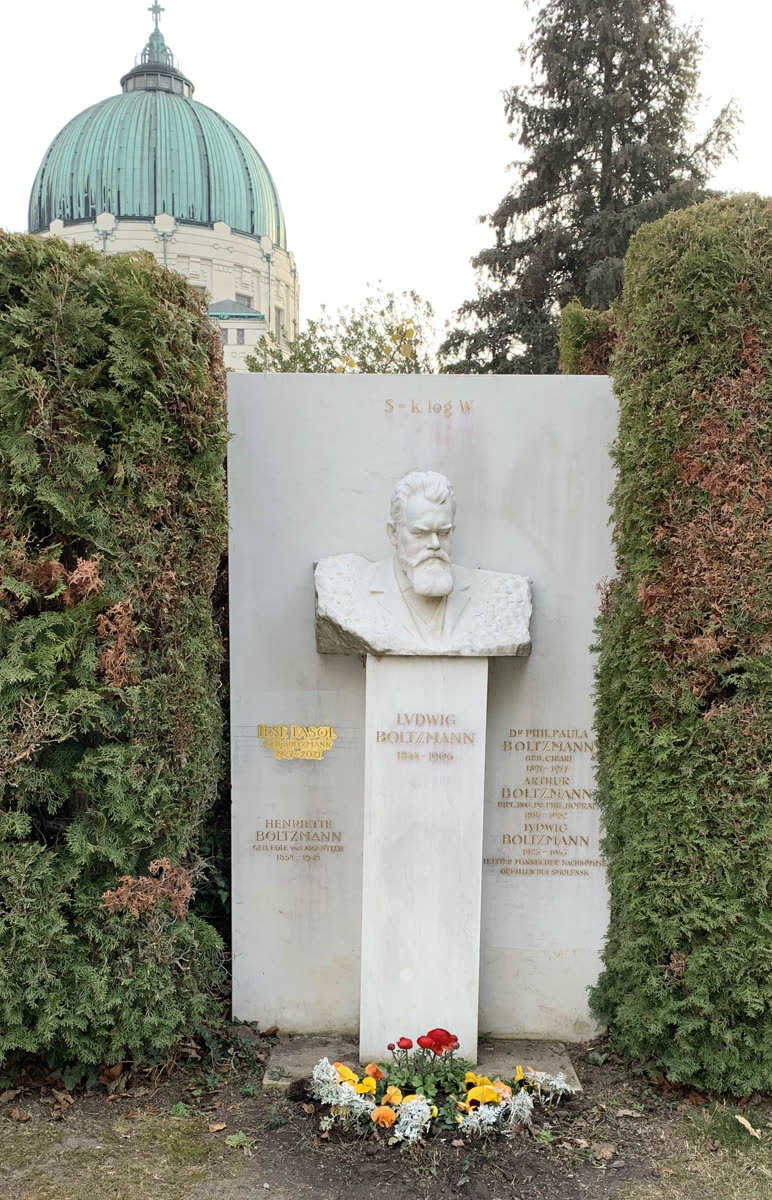
\includegraphics[width=\linewidth]{images/book4/boltzmann-grave.jpg}\par
{\footnotesize बोल्ट्समान की समाधि।}
\end{minipage}
\end{history}

\section{अभ्यास}

\begin{exercise}[$\star$]\label{exo:b3:partition-functions:1}
चार दोलित्र चार क्वांटम बाँटते हैं। वितरण सूचीबद्ध कीजिए, हर एक का भार दीजिए,
और जाँचिए कि उनका योग चार
\omterm{def:b3:many-electron-atoms:indistinguishable}{अविभेद्य} क्वांटमों को चार दोलित्रों में रखने के तरीकों की संख्या, $\binom{7}{3}$, है। कौन-से वितरण
सबसे प्रायिक हैं?
\end{exercise}

\begin{exercise}[$\star$]\label{exo:b3:partition-functions:2}
दो अनपभ्रष्ट स्तर \qty{2.5}{kJ/mol} दूर हैं। \qty{298.15}{K} पर और \qty{1000}{K} पर उनकी
\omterm{def:b3:partition-functions:boltzmann}{समष्टियों} का अनुपात परिकलित कीजिए। बहुत ऊँचे ताप पर सीमा
क्या है?
\end{exercise}

\begin{exercise}[$\star$]\label{exo:b3:partition-functions:3}
% ledger: aw:Ar
\qty{298.15}{K} पर आर्गन परमाणु का \omterm{def:b3:partition-functions:thermal-wavelength}{तापीय तरंगदैर्घ्य} और \qty{1}{dm^3} आयतन में
उसका स्थानांतरणीय विभाजन फलन परिकलित कीजिए।
\end{exercise}

\begin{exercise}[$\star$]\label{exo:b3:partition-functions:4}
% ledger: diat:N2.Be, diat:N2.ae, diat:HCl.Be, diat:HCl.ae
$B_0 = \qty{1.990}{cm^{-1}}$ (\ce{N2}) और \qty{10.440}{cm^{-1}} (\ce{H^{35}Cl}) के साथ हर अणु का $\theta_{\mathrm R}$ और
\qty{298.15}{K} पर उच्च-ताप घूर्णी विभाजन फलन
परिकलित कीजिए।
\end{exercise}

\begin{exercise}[$\star\star$]\label{exo:b3:partition-functions:5}
% ledger: diat:I2.we, diat:I2.wexe, diat:N2.we, diat:N2.wexe
\ce{I2} और \ce{N2} की मूल तरंग-संख्याएँ \qty{213.27}{cm^{-1}} और
\qty{2329.92}{cm^{-1}} हैं। $\theta_{\mathrm V}$, \qty{298.15}{K} पर $q^{\mathrm V}$, और उन अणुओं का अंश परिकलित कीजिए
जो $v = 0$ में नहीं हैं।
\end{exercise}

\begin{exercise}[$\star\star$]\label{exo:b3:partition-functions:6}
% ledger: diat:NO.split, lev:Cl.2P1_2
\qty{298.15}{K} पर \ce{NO} (\qty{119.73}{cm^{-1}} दूर स्थित दो द्वि-अपभ्रष्ट
स्तर) और क्लोरीन परमाणु (${}^2P_{3/2}$
मूल स्तर, ${}^2P_{1/2}$, \qty{882.35}{cm^{-1}} पर) का इलेक्ट्रॉनिक विभाजन फलन परिकलित कीजिए। \ce{NO} अणुओं का कितना अंश
ऊपरी स्तर में है? उच्च ताप पर $q^{\mathrm E}(\ce{NO})$ किसकी ओर प्रवृत्त होता है?
\end{exercise}

\begin{exercise}[$\star\star$]\label{exo:b3:partition-functions:7}
$q^{\mathrm T} = V/\Lambda^3$ से एकपरमाणुक आदर्श गैस के एक मोल की आंतरिक ऊर्जा और
स्थिर आयतन पर ऊष्मा धारिता व्युत्पन्न कीजिए, और \qty{298.15}{K} पर $U - U(0)$ का मान
निकालिए।
\end{exercise}

\begin{exercise}[$\star\star$]\label{exo:b3:partition-functions:8}
% ledger: aw:Ar, s0:Ar_g
सैकुर--टेट्रोड समीकरण से \qty{298.15}{K} पर आर्गन की मानक मोलर एन्ट्रॉपी
परिकलित कीजिए; सारणीबद्ध
\qty{154.846}{J.K^{-1}.mol^{-1}} से तुलना कीजिए। यदि दाब को 10 से भाग दिया जाए तो यह कितनी बदलती है?
\end{exercise}

\begin{exercise}[$\star\star$]\label{exo:b3:partition-functions:9}
% ledger: diat:HCl.Be, diat:HCl.ae
\qty{298.15}{K} पर \ce{H^{35}Cl} की मानक मोलर एन्ट्रॉपी में घूर्णी योगदान
परिकलित कीजिए ($\theta_{\mathrm R} = \qty{15.02}{K}$)।
\end{exercise}

\begin{exercise}[$\star\star\star$]\label{exo:b3:partition-functions:10}
$J$ को संतत मानकर दिखाइए कि रैखिक अणु का सबसे अधिक समष्टित घूर्णी स्तर
$J_{\max} = \sqrt{T/2\theta_{\mathrm R}} - \frac12$ के निकट है। \qty{300}{K} पर \ce{HCl}
($\theta_{\mathrm R} = \qty{15.02}{K}$) और \ce{CO} ($\theta_{\mathrm R} = \qty{2.766}{K}$) के लिए इसका मान निकालिए। अवरक्त बैंड की दोनों
शाखाएँ केंद्र से कुछ रेखाएँ दूर सबसे प्रबल क्यों होती हैं?
\end{exercise}

\begin{exercise}[$\star\star\star$]\label{exo:b3:partition-functions:11}
% ledger: diat:H2.Be, diat:H2.ae
ऑयलर--मैक्लॉरिन सूत्र $\sum_{J\ge0}f(J) \approx \int_0^\infty f(J)\dd J + \frac12f(0) -
\frac1{12}f'(0)$ देता है। इसे $f(J) = (2J+1)\eu^{-\theta J(J+1)/T}$ पर लगाइए और दिखाइए कि $q^{\mathrm R} \approx T/\theta +
\frac13$। किन तापों के लिए $T/\theta$, 1\,\% तक सही है? क्या यह \qty{298.15}{K} पर \ce{H2}
($B_0 = \qty{59.32}{cm^{-1}}$) के लिए स्वीकार्य है?
\end{exercise}

\begin{exercise}[$\star\star\star$]\label{exo:b3:partition-functions:12}
% ledger: diat:I2.we, diat:I2.wexe
दिखाइए कि कंपनिक मोलर एन्ट्रॉपी शून्य की ओर प्रवृत्त होती है जब $T \ll \theta_{\mathrm V}$, और
$R[1 + \ln(T/\theta_{\mathrm V})]$ की ओर जब $T \gg \theta_{\mathrm V}$। \qty{298.15}{K} पर \ce{I2}
($\theta_{\mathrm V} = \qty{306.9}{K}$) के लिए यथार्थ व्यंजक और यह सीमा दोनों निकालिए, और टिप्पणी कीजिए।
\end{exercise}

\section{समस्या: नाइट्रोजन की एन्ट्रॉपी की गिनती}

\begin{problem}[{सप्ताहांत समस्या --- नाइट्रोजन की एन्ट्रॉपी की गिनती: उसकी
मानक एन्ट्रॉपी में स्थानांतरणीय, घूर्णी, कंपनिक और इलेक्ट्रॉनिक योगदान,
उसके स्पेक्ट्रम से परिकलित और सारणी से तुलनित}]
\label{pb:b3:partition-functions:1}
% ledger: aw:N, diat:N2.Be, diat:N2.ae, diat:N2.we, diat:N2.wexe, s0:N2_g, const:h, const:kB, const:NA, const:c
नाइट्रोजन वायु की मुख्य गैस है। \qty{298.15}{K} पर उसकी मानक मोलर एन्ट्रॉपी
यहाँ उसके मोलर द्रव्यमान, \qty{28.014}{g/mol}, और उसके
स्पेक्ट्रमी स्थिरांकों से परिकलित की जाती है: $B_e = \qty{1.998241}{cm^{-1}}$, $\alpha_e = \qty{0.017318}{cm^{-1}}$, $\omega_e =
\qty{2358.57}{cm^{-1}}$, $\omega_ex_e = \qty{14.324}{cm^{-1}}$; उसका इलेक्ट्रॉनिक मूल पद ${}^1\Sigma_g^+$ है।
मानक दाब $p^\circ = \qty{1}{bar}$; $k = \qty{1.380649e-23}{J/K}$, $h = \qty{6.62607015e-34}{J.s}$।

\medskip\noindent\textbf{भाग I --- स्थानांतरण।}
\begin{enumerate}
  \item एक अणु का द्रव्यमान परिकलित कीजिए।
  \item \qty{298.15}{K} पर उसका \omterm{def:b3:partition-functions:thermal-wavelength}{तापीय तरंगदैर्घ्य} परिकलित कीजिए।
  \item प्रति अणु उपलब्ध आयतन, $kT/p^\circ$, परिकलित कीजिए।
  \item $q^{\mathrm T}/N$ निकालिए, और उसके आकार पर टिप्पणी कीजिए।
  \item स्थानांतरणीय मोलर एन्ट्रॉपी परिकलित कीजिए।
  \item आधे दाब पर यह कितनी बदलती?
\end{enumerate}

\medskip\noindent\textbf{भाग II --- घूर्णन।}
\begin{enumerate}[resume]
  \item $B_0$ परिकलित कीजिए।
  \item $\theta_{\mathrm R}$ परिकलित कीजिए।
  \item \omterm{def:b3:partition-functions:symmetry-number}{सममिति संख्या} दीजिए और बताइए कि वह किसका ध्यान रखती है।
  \item \qty{298.15}{K} पर $q^{\mathrm R}$ परिकलित कीजिए।
  \item क्या उच्च-ताप रूप उचित है?
  \item घूर्णी मोलर एन्ट्रॉपी परिकलित कीजिए।
  \item नाभिकीय-चक्रण भारों की उपेक्षा करते हुए, कौन-सा घूर्णी स्तर सबसे अधिक
        समष्टित है?
\end{enumerate}

\medskip\noindent\textbf{भाग III --- कंपन और इलेक्ट्रॉनिक अवस्थाएँ।}
\begin{enumerate}[resume]
  \item कंपनिक क्वांटम $G(1) - G(0)$ परिकलित कीजिए।
  \item $\theta_{\mathrm V}$ परिकलित कीजिए।
  \item \qty{298.15}{K} पर $q^{\mathrm V}$ परिकलित कीजिए।
  \item अणुओं का कितना अंश $v = 1$ में है?
  \item कंपनिक मोलर एन्ट्रॉपी परिकलित कीजिए।
  \item इलेक्ट्रॉनिक योगदान क्या है? उत्तेजित इलेक्ट्रॉनिक अवस्थाओं की उपेक्षा क्यों
        की जा सकती है?
\end{enumerate}

\medskip\noindent\textbf{भाग IV --- योग और तुलना।}
\begin{enumerate}[resume]
  \item योगदानों को जोड़िए।
  \item सारणीबद्ध \qty{191.609}{J.K^{-1}.mol^{-1}} से तुलना कीजिए।
  \item किसी सारणी का ऊष्मामितीय मान किन मापनों पर आधारित है?
  \item सारणियाँ नाभिकीय चक्रण को क्यों छोड़ सकती हैं?
  \item परिणाम बताइए: स्पेक्ट्रमी स्थिरांकों से परिकलित, \qty{298.15}{K} पर नाइट्रोजन की
        मानक मोलर एन्ट्रॉपी।
\end{enumerate}
\end{problem}
